%; whizzy chapter -dvi
% -initex iniptex -latex platex -format platex -bibtex jbibtex -fmt fmt
% $B0J>e(B whizzytex $B$r;HMQ$9$k>l9g$N@_Dj!#(B
 
%     Tokyo Debian Meeting resources
%     Copyright (C) 2012 Junichi Uekawa
%     Copyright (C) 2011 Nobuhiro Iwamatsu

%     This program is free software; you can redistribute it and/or modify
%     it under the terms of the GNU General Public License as published by
%     the Free Software Foundation; either version 2 of the License, or
%     (at your option) any later version.

%     This program is distributed in the hope that it will be useful,
%     but WITHOUT ANY WARRANTY; without even the implied warranty of
%     MERCHANTABILITY or FITNESS FOR A PARTICULAR PURPOSE.  See the
%     GNU General Public License for more details.

%     You should have received a copy of the GNU General Public License
%     along with this program; if not, write to the Free Software
%     Foundation, Inc., 51 Franklin St, Fifth Floor, Boston, MA  02110-1301 USA

%  preview (shell-command (concat "evince " (replace-regexp-in-string "tex$" "pdf"(buffer-file-name)) "&"))

%%$B$3$3$+$i%X%C%@3+;O!#(B

\documentclass[mingoth,a4paper]{jsarticle}
\usepackage{monthlyreport}
% $BF|IU$rDj5A$9$k!"Kh7nJQ$o$j$^$9!#(B
\newcommand{\debmtgyear}{2014}
\newcommand{\debmtgmonth}{04}
\newcommand{\debmtgdate}{19}
% started from zero:
% (let ((year 2013) (month 7)) (+ (* (- year 2005) 12) month -1))
\newcommand{\debmtgnumber}{112}

\begin{document}

\begin{titlepage}
\thispagestyle{empty}
% $B%?%$%H%k%Z!<%8(B:$BJT=8I,MW$JItJ,$O:G=i$N%^%/%m$KHt$P$9$3$H(B

\vspace*{-2cm}
$BBh(B\debmtgnumber{}$B2s(B $BEl5~%(%j%"(B Debian $BJY6/2q;qNA(B\\
\hspace*{-2cm}

\includegraphics{image2012-natsu/dotdeb.pdf}\\
\hfill{}\debmtgyear{}$BG/(B\debmtgmonth{}$B7n(B\debmtgdate{}$BF|(B

% $B$3$3$O%"%C%W%G!<%H$9$k$3$H(B
% $BA43QJ8;z$K$7$J$$$H%U%)%s%H$N%5%$%:$,9g$o$J$$$N$GCm0U(B
\rotatebox{10}{\fontsize{32}{32} {\gt $BFC=8!'(BGolang$B$J%D!<%k$N%Q%C%1!<%82=(B}}\\
\rotatebox{10}{\fontsize{32}{32} {\gt (Serf$BJT(B)}}\\

\vspace*{-2cm}
\hfill{}
\includegraphics[height=6cm]{image200502/openlogo-nd.eps}
\end{titlepage}

\newpage

\begin{minipage}[b]{0.2\hsize}
 \definecolor{titleback}{gray}{0.9}
 \colorbox{titleback}{\rotatebox{90}{\fontsize{80}{80} {\gt $B%G%S%"%sJY6/2q(B} }}
\end{minipage}
\begin{minipage}[b]{0.8\hsize}
\hrule
\vspace{2mm}
\hrule
\begin{multicols}{2}
\tableofcontents
\end{multicols}
\vspace{2mm}
\hrule
\end{minipage}

\dancersection{$B;vA02]Bj(B}{$BLnEg(B $B5.1Q(B}

$B:#2s$N;vA02]Bj$O0J2<$G$9(B:
\begin{enumerate}
 \item $BK\F|!"2?$N:n6H$r$d$k$+$r@k8@$/$@$5$$!#(B
\end{enumerate}
$B$3$N2]Bj$KBP$7$FDs=P$$$?$@$$$?FbMF$O0J2<$G$9!#(B
\begin{multicols}{2}
{\small
\begin{prework}{ 野島貴英 }

\begin{itemize}
\item Xmrisパッケージ化頑張る
\item iOS7.1 debian接続再び。
\end{itemize}
\end{prework}

\begin{prework}{ 岩松 信洋 }

?

\end{prework}

\begin{prework}{ dictoss(杉本 典充) }

Debian上でLeap Motionを動かしてみる

\end{prework}

\begin{prework}{ Yoshida Shin }

GitHub に公開しているプログラムの機能追加。
動作環境は Debian Sid で。
\end{prework}

\begin{prework}{ Koji Hasebe }

Debianパッケージ作成の方法を調査し、実際に作成する。
アウトプットとして、その方法を手順書にまとめる。
\end{prework}

\begin{prework}{ henrich }
\begin{itemize}
\item OSC北海道用の資料作成
\item debhelperの査読の続き
\item パッケージまわりでのなにか
\end{itemize}
のいずれか。

\end{prework}

\begin{prework}{ zinrai }

Debianパッケージ作成。
\begin{itemize}
\item Debianパッケージ作成してみたい
\item 「Debianパッケージング道場」に都合がつかず参加できなかったので「もくもく会」の時間を使いパッケージ作成の作法を心得ている人がいる環境でパッケージ作成したい
\item redis 2.8.8をDebianパッケージ作成の題材にしてみようと思う。
\url{http://redis.io/}
\item 通勤時間などを使い当日までにこの辺に目を通しておきたい
\url{http://www.debian.or.jp/community/devel/}
\end{itemize}
\end{prework}

\begin{prework}{ yyuu }

自分で管理してるプロジェクトのdeb化を要望されてしまったので、そのための作業を行ないたいと考えています。

\url{https://github.com/yyuu/pyenv/issues/138}

\end{prework}

\begin{prework}{ 野首(@knok) }
\begin{itemize}
\item KAKASIローマ字テーブルの改善
\item LanguageToolのルール追加
\item gnu.org, veの翻訳
\end{itemize}
\end{prework}

\begin{prework}{ まえだこうへい }

\begin{itemize}
\item Golang関係のパッケージ化の話をする
\item \url{http://qa.debian.org/developer.php?login=mkouhei@palmtb.net}
のバグ潰し&パッケージアップデート
\item 上記のGolang関係のパッケージをpkg-go teamでのメンテナンスを始める(MLに投稿&ITPする)
\end{itemize}
\end{prework}

}
\end{multicols}

\dancersection{Debian Trivia Quiz}{$BLnEg(B $B5.1Q(B}

$B$H$3$m$G!"$_$J$5$s(B Debian $B4XO"$NOCBj$K$*$$$D$$$F$$$^$9$+!)(BDebian$B4XO"$NOC(B
$BBj$O%a!<%j%s%0%j%9%H$r$h$s$G$$$k$HDI@W$G$-$^$9!#$?$@$h$s$G$$$k$@$1$G$O$O(B
$B$j$"$$$,$J$$$N$G!"M}2rEY$N%F%9%H$r$7$^$9!#FC$K0l?M$@$1$G$O0UL#$,$o$+$i$J(B
$B$$$H$3$m$b$"$k$+$bCN$l$^$;$s!#$_$s$J$G0l=o$KFI$s$G$_$^$7$g$&!#(B

$B:#2s$N=PBjHO0O$O(B\url{debian-devel-announce@lists.debian.org} $B$d(B \url{debian-devel@lists.debian.org}$B$KEj9F$5$l$?(B
$BFbMF$J$I$+$i$G$9!#(B

\begin{multicols}{2}
%; whizzy-master ../debianmeetingresume201311.tex
% $B0J>e$N@_Dj$r$7$F$$$k$?$a!"$3$N%U%!%$%k$G(B M-x whizzytex $B$9$k$H!"(Bwhizzytex$B$,MxMQ$G$-$^$9!#(B
%

\santaku
{2015$BG/$N(BDebconf15$B$N3+:E9q$O$I$3$K$J$C$?$G$7$g$&!)(B}
{$B%\%9%K%"!&%X%k%D%'%4%S%J(B}
{$B%&%/%i%$%J(B}
{$B%I%$%D(B}
{C}
{$B:#EY$O%I%$%D$@$=$&$G$9!#$A$J$_$K:#G/$N(BDebconf14$B$O(B8/23-31$B$G(BUSA$B$N(BPortland,Oregon
$B$G3+:EM=Dj$G$9!#(B}

\santaku
{DPL$BA*5s$,9T$o$l$^$7$?!#:#G/$N(BDPL$B$OC/$K$J$C$?$G$7$g$&$+!)(B}
{Lucas Nussbaum}
{Neil McGovern}
{Rapha\"{e}l Hertzog}
{A}
{$B:#G/$N(BDPL$B$N8uJd<T$O#2L>$G!"(BLucas Nussbaum$B$5$s!"(BNeil McGovern$B$5$s$N#2L>(B
$B$G$7$?!##2L>$H$b<+A&$H$N$3$H$G$9!#A*5s$N7k2L!"(B
Lucas Nussbaum(lucus)$B$5$s$N05>!$@$C$?$h$&$G$9!#$A$J$_$K!"(B
Rapha\"{e}l Hertzog$B$5$s$O!"(BThe Debian 
Administrator\'s handbook$B$N:n<T!"B>$K$b0N6H$,$?$/$5$s!#(B}

\santaku
{clang3.4$B$K$h$k(BDebian$B%Q%C%1!<%8$N:F9=C[$,9T$o$l$^$7$?!#7k2L2?(B\%$B$N%Q%C%1!<%8$,@.8y$7$?$G$7$g$&$+!)(B}
{90\%}
{50\%}
{10\%}
{A}
{\url{http://clang.debian.net/}$B$,(Bclang$B$K$h$k(BDebian$B%Q%C%1!<%8:F9=C[$N%]!<%?%k%5%$%H$G$9!#KhG/!"(Bclang$B$N%P!<%8%g%s$r>e$2$F!"A4(BDebian$B%Q%C%1!<%8$r:F9=C[$7$?7k2L$,:\$j$^$9!#:#G/$N7k2L$H$7$F$O:F9=C[BP>]$N%Q%C%1!<%8$N?t$,5nG/$HBgI}$KA}$($F$$$k$K$b$+$+$o$i$:!"9=C[<:GT$K=*$o$C$?%Q%1!<%8?t$,5nG/$HJQ$o$i$J$+$C$?$H$$$&Hs>o$KNI$$7k2L$H$J$C$F$$$^$9!#(B}

\santaku
{beagle board$B%7%j!<%:$H$$$&Hs>o$K?M5$$N$"$k(BARM$B$N<B83%\!<%I$K%P%s%I%k$5$l$k(BOS$B$N>-Mh$N8+DL$7$K$D$$$F!"(Bbeagle board$B$NAON)<T$,$I$N(BOS$B$K$9$kM=Dj$HH/8@$7$?$+!)(B}
{Gentoo}
{Debian$B$C$7$g!*(BDebian}
{Andoroid OS}
{B}
{\url{http://opensource.com/life/14/3/interview-jason-kridner-beagleboard}
$B$K$F!">-Mh(BDebian$B$K$9$k$H$$$&H/8@$,$"$j$^$9!#$H$3$m$G!"(Bbeagle board$B%7%j!<%:$OL$$@$K(BOMAP$B$r(B
$B;H$$B3$1$k$N$+$,6=L#DE!9$G$O$"$j$^$9!#(B}

\santaku
{$B7cO@$NKv!"(B3$B7nCf=\:"$K(BDebian$B$N(Bca-certificates$B%Q%C%1!<%8$+$i>C$($?(Broot$B>ZL@=q$,$"$j$^$9!#$=$l$O$J$s$G$7$g$&!)(B}
{RapidSSL$B$N(Broot$B>ZL@=q(B}
{CAcert$B$N(Broot$B>ZL@=q(B}
{Verisign$B$N(Broot$B>ZL@=q(B}
{B}
{$B5DO@$N%5%^%j$O!"(BLWN$B$N5-;v(B\url{https://lwn.net/Articles/590879/}$B$,H=$j$d$9$$$G$9!#$^$?!"(BCAcert$B$C$F2?!)$H$$$&J}$O!"Bh(B71$B2sEl5~%(%j%"(BDebian$BJY6/2q(B(2010$BG/(B12$B7n3+:E(B)\url{http://tokyodebian.alioth.debian.org/2010-12.html}$B$K7G:\$5$l$F$$$kJY6/2q;qNA$,$*4+$a$G$9!#(B}

\santaku
{Jessie$B$K$F%G%9%/%H%C%W4D6-$rA*Br$7$?:]$KF3F~$5$l$k!"%G%U%)%k%H%3%_%e%K%1!<%7%g%s%D!<%k$N8uJd$K$D$$$F5DO@$,$5$l$F$$$j$^$9!#0J2<$N$I$l$G$7$g$&!)(B}
{Empathy}
{licq}
{jitsi}
{C}
{Debian$B$G$O!"%G%U%)%k%H$N%3%_%e%K%1!<%7%g%s%D!<%k$H$7$F!"$[$\40A4$K(BRTC/VoIP$B$r%5%]!<%H$9$k$3$H$,K>$^$7$$$H$5$l$?$?$a!"$3$A$i$K8~$$$F$$$k%D!<%k$H$7$F:#$^$G$N(BEmpathy$B$h$j$b(Bjitsi$B$,8~$$$F$$$k$N$G$O!)$H$$$&$3$H$+$i5DO@$,3+;O$5$l$^$7$?!#(B}

\santaku
{$B@hF|(BDebian$B$K(BOTR$B%A!<%`$H$$$&(BOTR$B%=%U%H$r%Q%C%1!<%82=$9$k%0%k!<%W$,7k@.$5$l$^$7$?!#$H$3$m$G(BOTR$B$C$F$J$s$NN,!)(B}
{Owa-Tte-Ru}
{OpticalTRacking}
{Off-the-Record}
{C}
{Off-the-Record$B$H$O!"0E9f2=5;=Q$r;H$C$F%$%s%U%iDs6!<T$K$9$i%a%C%;!<%8$N$d$j$H$j$NFbMF$r8+$;$J$$!J5-O?$5$;$J$$!K%a%C%;!<%8%5!<%S%9$rL\;X$7$?$b$N$G$9(B\url{https://www.otr.im/}$B!#(B}

\santaku
{$B@hF|!"(BDebian squeeze$B$N%5%]!<%H4|4V$,?-$S$k@k8@$,(BDSA$B$K$h$j%"%J%&%s%9$5$l$^$7$?!#7k6I$$$D$K$J$C$?!)(B}
{2015/2}
{2016/2}
{2016/5}
{B}
{Long Term Support(LTS)$B$@$=$&$G$9(B\url{https://lists.debian.org/debian-security-announce/2014/msg00082.html}$B!#M=Dj$G$O!"(B2014/5/31$B:"$K%5%]!<%H=*N;$9$k$O$:$G$7$?$N$G!"#2G/<e$N1dD9$H$J$j$^$9!#$?$@%5%]!<%H1dD9$5$l$k$N$O!"(BDebian squeeze$B$NA4It$N%Q%C%1!<%8$G$O$J$$$N$G!"%5%]!<%H$5$l$J$$%Q%C%1!<%8$r==J,$K$*;H$$$N3'MM$O!"(BDebian wheezy$B$X%"%C%W%0%l!<%I$9$k$3$H$r$*4+$a$7$F$*$-$^$9!#(B}



\end{multicols}

\dancersection{$B:G6a$N(BDebian$B4XO"$N%_!<%F%#%s%0Js9p(B}{$BLnEg(B $B5.1Q(B}

\subsection{$BEl5~%(%j%"(BDebian$BJY6/2q(B111$B2sL\Js9p(B}

 $BEl5~%(%j%"(BDebian$BJY6/2q(B111$B2sL\$O(B($B3t(B)$B%9%/%&%'%"!&%(%K%C%/%9$5$s$G3+:E$5$l$^$7$?!#(B
5$BL>$N;22C<T$,$"$j$^$7$?!#(B

\begin{itemize}
\item debian$B$+$i(Biphone5(iOS7.1)$B$K$D$J$07o$K$D$$$F!"(B
  \begin{itemize}
    \item debian$B%Q%C%1!<%8$r:n$C$F$D$J$.!"(B
    \item $B8x3+>pJs$K4p$E$$$?@\B35;=Q(B
$B!!(B\end{itemize}
$B$K$D$$$FH/I=$,$"$j$^$7$?!#(B
\item $B;22C<TA40w$G!"3F<+$N:n6H$r9T$$!":G8e$K@.2LH/I=$r$7$^$7$?!#(B
\end{itemize}

% % (query-replace-regexp "<.*?>" "")
% % (query-replace-regexp "^[	 ]\+" "")

%-------------------------------------------------------------------------------
\dancersection{Golang$B$G=q$+$l$?%D!<%k$r(BDebian$B%Q%C%1!<%8$K$9$k(B}{$BA0ED(B $B9LJ?(B}
%-------------------------------------------------------------------------------
\index{Golang}
\index{dh-golang}

\subsection{$B$O$8$a$K(B}

$B$"$k$3$H$r$d$k$N$K(BSerf\footnote{\url{http://www.serfdom.io/}}$B$H$$$&%D!<%k$,NI$$$N$G$O!"$HF1N=$K=u8@$r$b$i$C$?$N$G!"(BSerf$B$G$d$j$?$$$3$H$,$G$-$J$$$+8!>Z$r$9$k$3$H$K$7$^$7$?!#$G$9$,!"$=$b$=$b(BDebian$B%Q%C%1!<%8$K$OL5$$$N$G$^$:$=$3$+$i$G$7$g!"$H$$$&$3$H$G<j85$G(BDebian$B%Q%C%1!<%8$K$7$^$7$?!#(B\footnote{Serf$B<+BN$N$*OC$rJ9$-$?$$$H;W$C$?J}$O;DG0!#(BUpstream\footnote{\url{https://github.com/hashicorp/serf/}}$B$N%I%-%e%a%s%H$dF|K\8l$N(BSerf$B$r;H$C$?%*!<%1%9%H%l!<%7%g%s$N;qNA$r8+$?$@$1$G!"(BSerf$B<+BN$N8!>Z$O$^$@9T$C$F$$$J$$$N$G!"(BSerf$B$=$N$b$N$K$D$$$F$O2?$b8l$l$^$;$s!#(B}

Serf$B$r(BDebian$B%Q%C%1!<%8$K$9$k$K$"$?$j!"9T$C$?$3$H$d!"(BGolang$B$N%D!<%k$r(BDebian$B%Q%C%1!<%8$K$9$k>e$GI,MW$JCN<1!"<j=g$r$^$H$a$^$7$?!#:#2s$NJY6/2q$G$O!"(BDebian$B%Q%C%1!<%8$r=i$a$F:n@.$9$k?M$N3d9g$,Hf3SE*B?$+$C$?$N$G!"FbMFE*$K>/$7>iD9$K$J$C$F$$$^$9!#(B

\subsection{Debian$B$G$N(BGolang$B$N4D6-9=C[(B}

\subsubsection{$BA0Ds>r7o(B}

$B;HMQ$9$k%G%#%9%H%j%S%e!<%7%g%s$O!"(BDebian GNU/Linux Sid$B$rA0Ds$H$7$^$9!#<j85$K(BSid$B$N4D6-$,$J$$>l9g$O!"2>A[%^%7%s$J$I$GMQ0U$7$F$/$@$5$$!#(B

\subsubsection{Debian$B%Q%C%1!<%8$N%$%s%9%H!<%k(B}

Debian$B$G$O!"(B ``golang'' $B$H$$$&%a%?%Q%C%1!<%8$,MQ0U$5$l$F$$$^$9!#$3$l$r%$%s%9%H!<%k$9$k$H<!$N%Q%C%1!<%8$,%$%s%9%H!<%k$5$l$^$9!#(B\footnote{Linux Kernel$B$N(B amd64$B%"!<%-%F%/%A%c$N>l9g(B}

\begin{itemize}
\item golang-doc \\
  \url{http://golang.org}$B$N%I%-%e%a%s%H!#(B\texttt{godoc --http=:6060} $B$r<B9T$7!"(B\url{http://localhost:6060/}$B$G1\Mw2D(B
\item golang-go \\
  Golang$B$N%"%;%s%V%i!"%3%s%Q%$%i!<!"%j%s%+!<$J$I$N%D!<%k%A%'%$%s(B
\item golang-go-linux-amd64 \\
  Linux$B%7%9%F%`!"(Bamd64$B%"!<%-%F%/%A%c8~$1$NI8=`%i%$%V%i%j!#(Bsystem: darwin,freebsd,linux,netbsd,windows$B!"(Barch: amd64,386,arm
\item golang-go.tools \\
  Golang$BMQ$NJd=u%D!<%k!#A0=R$N(Bgodoc$B%3%^%s%I$b4^$^$l$k(B
\item golang-src \\
  golang$B%Q%C%1!<%8$N%=!<%9%3!<%I!#(Bgodoc$B%3%^%s%I$J$I$G;H$o$l$k(B
\item libjs-jquery \\
  jQuery$B!#(Bgolang-go.tools$B$K0MB8!#(Bgodoc$B%3%^%s%I$G<B9T$9$k(Bgolang-doc$B$N%I%-%e%a%s%HMQ(B
\item javascript-common \\
  JavaScript$B%i%$%V%i%j%Q%C%1!<%8$N%5%]!<%H%Q%C%1!<%8!#(Blibjs-jquery$B$K0MB8(B
\end{itemize}

\subsection{Golang$B$N%3%s%Q%$%kJ}K!(B}

$BI8=`%i%$%V%i%j$N$_$G=q$+$l$?%3!<%I$r%3%s%Q%$%k$9$k>l9g$K$O!"(B\texttt{go build}$B%3%^%s%I$N$_$G$G$-$^$9!#(B
$BNc$($P!"$*$J$8$_$K(BHello world$B$N%3!<%I(B(hello.go)$B$rMQ0U$7$^$9!#(B

\begin{commandline}
package main

import "fmt"

func main() {
  fmt.Println("Hello world.")
}
\end{commandline}

$B%3%s%Q%$%k$7$^$9!#(B

\begin{commandline}
$ go build hello.go

\end{commandline}

$B%P%$%J%j$N<B9T$O(B\texttt{./hello}$B$G$9!#(B

\begin{commandline}
$ ./hello
Hello world.
\end{commandline}

\texttt{file}$B%3%^%s%I$G8+$k$H!"@EE*%j%s%/$5$l$F$$$k$3$H$,J,$+$j$^$9!#(B

\begin{commandline}
$ file hello
hello: ELF 64-bit LSB executable, x86-64, version 1 (SYSV), statically linked, not stripped
\end{commandline}

$B$J$*!"(B\texttt{go run}$B%3%^%s%I$r;H$&$H!"%3%s%Q%$%k$7$J$/$F$b<B9T2DG=$G$9!#(B
\begin{commandline}
$ rm hello
$ go run hello.go
Hello world.
$ ls hello
ls: cannot access hello: No such file or directory
\end{commandline}

\subsubsection{$BI8=`%i%$%V%i%j0J30$K0MB8$9$k(BGolang$B%Q%C%1!<%8$N%3%s%Q%$%k(B}

$B$^$:!"0MB8$9$k%Q%C%1!<%8$NG[CV>l=j$r4D6-JQ?t(B\texttt{GOPATH}$B$G;XDj$9$kI,MW$,$"$j$^$9!#(B

$B%7%9%F%`%0%m!<%P%k$N@_Dj$O!"(BDebian$B$G$O!"(B\texttt{/usr/share/gocode}$B$K$J$j$^$9!#4{$K(BDebian$B%Q%C%1!<%8$K$J$C$F$$$k(BGolang$B$N%i%$%V%i%j$O!"$3$N%G%#%l%/%H%j$N2<$K$"$k!"(Bsrc$B%G%#%l%/%H%j0J2<$K%$%s%9%H!<%k$5$l$^$9!#(B

$B%7%9%F%`%0%m!<%P%k$G@_Dj$5$l$F$$$k%Q%C%1!<%8$r;H$&>l9g$K$O!"(B

\begin{commandline}
$ export GOPATH=/usr/share/gocode
\end{commandline}

GOPATH$B$O@dBP%Q%9$G;XDj$9$kI,MW$,$"$j$^$9!#(B
$B%3%s%Q%$%k$9$k%3!<%I$HF1$8%+%l%s%H%G%#%l%/%H%j$KB8:_$9$k$J$i!"(B
\begin{commandline}
$ export GOPATH=$(pwd)
\end{commandline}

$B$H<B9T$7$?>e$G!"<B:]$N%Q%C%1!<%8$NG[CV$O!"(B
\texttt{\$(pwd)/src/example.org/mkouhei/hoge/}$B$N$h$&$J%G%#%l%/%H%j9=@.$K$J$C$F$$$kI,MW$,$"$j$^$9!#(B
$B@h$[$I$N(Bhello.go$B$K$3$N%Q%C%1!<%8$r(Bimport$B$9$k>l9g!"(B

\begin{commandline}
import (
    "fmt"
    "example.org/mkouhei/hoge"
)
\end{commandline}

$B$N$h$&$K$J$j$^$9!#(B

$B$J$*!"I8=`%i%$%V%i%j$O!"(BDebian$B$G$O!"(B\texttt{/usr/lib/go}$B0J2<$K%$%s%9%H!<%k$5$l$F$$$^$9!#I8=`%i%$%V%i%j%i%$%V%i%j$O!"(BGOPATH$B$G;XDj$9$kI,MW$O$J$/!"(BGOROOT$B$H$$$&4D6-JQ?t$G!"(B\texttt{/usr/lib/go}$B$,@_Dj$5$l$F$$$^$9!#(B

GOPATH$B$,@_Dj$5$l$F$$$l$P!"%Q%C%1!<%8$N%@%&%s%m!<%I$H%$%s%9%H!<%k$O(B\texttt{go get}$B%3%^%s%I$G9T$($^$9!#(B\footnote{\url{http://golang.org/cmd/go/\#hdr-Download_and_install_packages_and_dependencies}}

\texttt{GOPATH}$B$G;XDj$7$?%G%#%l%/%H%j0J2<$K!"2<5-$N$h$&$J7A$G<+F0E*$K%$%s%9%H!<%k$5$l$^$9!#(B

\begin{commandline}
$ go get example.org/mkouhei/hoge
$ tree
.
|-- pkg
|   `-- linux_amd64
|       `-- example.org
|           `-- mkouhei
|               `-- hoge.a
`-- src
    `-- example.org
        `-- mkouhei
            `-- hoge
                |-- LICENSE
                |-- README.rst
                `-- hoge.go
\end{commandline}

\texttt{GOPATH}$B$r@_Dj$7!"(Bimport$B$G$-$l$P!"(B\texttt{go build}$B$O0MB84X78$r2r7h$7$F%3%s%Q%$%k$G$-$^$9!#(B
$B%P%$%J%j$N$_$r(BDebian$B%Q%C%1!<%8$K$9$k:]$K!"(B\texttt{GOPATH}$B$,=EMW$G$9!#(B

\subsection{Golang$B$G=q$+$l$?%=%U%H%&%'%"$N(BDebian$B%Q%C%1!<%8:n@.J}K!(B}

Golang$B$G=q$+$l$?%=%U%H%&%'%"$N(BDebian$B%Q%C%1!<%8:n@.J}K!$K$D$$$F@bL@$7$^$9!#(B
$BBg$-$/<!$N(B2$B%Q%?!<%s$,$"$j$^$9!#(B

\begin{itemize}
\item $B%P%$%J%j$N$_(B
\item $B%i%$%V%i%j$N$_!J$b$7$/$O%i%$%V%i%j$H%P%$%J%j!K(B
\end{itemize}

$BA0<T$G$O%3%s%Q%$%k$,I,MW$G$9!#(BGolang$B$N>l9g!"0MB8$9$k%i%$%V%i%j$rA4$F@EE*$K%j%s%/$9$k$?$a!"%P%$%J%j$N<B9T$=$N$b$N$K$O0MB84X78$O$"$j$^$;$s!#$G$9$N$G!"%G!<%b%s2=$9$k%1!<%9$G$J$1$l$P!"(BDepends$B$K5-=R$9$k%Q%C%1!<%8$,4pK\I,MW$"$j$^$;$s!#(B\footnote{$B%G!<%b%s2=$7$F(BOS$B5/F0;~$K<+F05/F0$9$k>l9g!"%m%0$N%m!<%F!<%7%g%s$G(Blogrotate$B$K0MB8$7$?$j!"@lMQ%f!<%6$r:n$C$F<B9T$5$;$k$N$K(Badduser$B$,I,MW$G$9!#(B}

$B8e<T$G$O!"4pK\E*$K$O%3%s%Q%$%k$=$N$b$N$OI,MW$"$j$^$;$s!#$7$+$7!"A0=R$N(B/usr/share/gocode$B2<$K%=!<%9%3!<%I$r%$%s%9%H!<%k$9$kI,MW$,$"$k$N$G!"(Bdh-golang$B%Q%C%1!<%8$r(BBuild-Depends$B5-=R$7!"(Bdebian/rules$B$G!"(B\texttt{dh}$B%3%^%s%I$K(B\texttt{--with=golang}$B%*%W%7%g%sEO$7$F$d$kI,MW$,$"$j$^$9!#(B

$B$^$?!"%P%$%J%j!"%i%$%V%i%j$KLd$o$:!"0MB8$9$k(BGolang$B$N%Q%C%1!<%8$rA4$F(BBuild-Depends$B$K5-=R$9$kI,MW$,$"$j$^$9!#(B\footnote{$B$3$l$O(BGolang$B$K8B$C$?OC$G$O$"$j$^$;$s$M!#(B}$B$^$?!"(BGolang$B$G$O(B\texttt{go test}$B$G%F%9%H$r<B9T$7$?$j!"(B\texttt{go build}$B$d(BMakefile$B$G%3%s%Q%$%k$9$k>l9g!"0MB8$9$k(BGolang$B%Q%C%1!<%8$r(B\texttt{go get}$B$G(BGOPATH$B$G;XDj$7$?%G%#%l%/%H%j$K%@%&%s%m!<%I$*$h$S%$%s%9%H!<%k$5$l$k$N$G$9$,!"(BDebian$B%Q%C%1!<%8$N%S%k%I$G$O!"(B\texttt{go get}$B$r;H$o$J$$$h$&$K$7$J$/$F$O$$$1$^$;$s!#(B

\subsubsection{Debian$B%Q%C%1!<%8:n@.MQ$N4D6-@_Dj(B}

$B$^$:(Bdh-golang$B%Q%C%1!<%8$r%$%s%9%H!<%k$7$^$9!#(BDebian$B%Q%C%1!<%8<+BN$r:n$C$?$3$H$,L5$/!"0l$+$i4D6-$r@0$($k!"$H$$$&?M$O!"<!$N%3%^%s%I$r<B9T$7$^$9!#(B

\begin{commandline}
$ sudo apt-get devscripts debhelper fakeroot dh-golang cowbuilder piuparts git git-buildpackage
\end{commandline}

git$B$*$h$S(Bgit-buildpackage\footnote{git-buildpackage$B$O%=!<%9%Q%C%1!<%8<+BN$r(BGit$B$G4IM}$9$k$?$a$N%D!<%k$G$9!#(B}$B$OI,?\$G$O$"$j$^$;$s!#$7$+$7!"(BGolang$B$G=q$+$l$?$N%D!<%k$NB?$/$O(BGit$B%j%]%8%H%j$G4IM}$5$l$F$$$^$9!#$^$?!"@N$J$,$i$N%P!<%8%g%K%s%0$,$5$l$J$$%1!<%9$,$[$H$s$I$G$9!#$=$N$?$a!"(Btarball$B<+BN$NDs6!$b$5$l$J$$$b$N$,B?$$$N$G!"(BGit$B$,DL>oI,MW$K$J$j$^$9!#(B

$B$^$?(BGolang$B$N(BDebian$B%Q%C%1!<%8$N%a%s%F%J%s%9%A!<%`(B(the pkg-go team\footnote{\url{http://pkg-go.alioth.debian.org/}})$B$G$O!"(Bgit-buildpackage$B$G%=!<%9%Q%C%1!<%8$r4IM}$9$k$3$H$K$J$C$F$$$^$9!#(B\footnote{\url{http://pkg-go.alioth.debian.org/packaging.html\#_packaging_in_git}}

$B$J$*!"A0=R$N(B\texttt{go get}$B%3%^%s%I$G$O!"%j%]%8%H%j$+$iF~<j$7$F!"$=$N$^$^(B\texttt{GOPATH}$B$G@_Dj$7$?%G%#%l%/%H%j$N(Bsrc$B%G%#%l%/%H%j0J2<$KE83+$5$l$F$7$^$&$N$G!"%P!<%8%g%s$d%3%_%C%H$,J,$+$i$J$$$N$G;H$o$J$$J}$,$h$$$G$7$g$&!#$J$*!"(BBuild-Depends$B$G$N0MB84X78$N2r7h$N:]$K$b!"(BDebian$B%Q%C%1!<%8%s%0%]%j%7!<>e!"(B\texttt{go get}$B%3%^%s%I$O;H$($^$;$s!#(B

.bashrc$B$K2<5-$N$h$&$JJQ?t$r@_Dj$7$^$9!#(B
\begin{commandline}
export DEBFULLNAME='Kouhei Maeda'
export DEBEMAIL=mkouhei@palmtb.net
\end{commandline}

pbuilder, cowbuilder$B$N(Bchroot$B%$%a!<%8$r:n@.$7$^$9!#(B\footnote{pbuilder$B$O(Bcowbuilder$B$r%$%s%9%H!<%k$9$k$H<+F0E*$K%$%s%9%H!<%k$5$l$^$9!#(B}

\begin{commandline}
$ sudo pbuilder --create
$ cowbuilder --create
\end{commandline}
pbuilder$B$NJ}$O!"(B/var/cache/pbuilder/base.tgz$B$,!"(Bcowbuilder$B$NJ}$O(B/var/cache/pbuilder/base.cow$B$,:n@.$5$l$^$9!#(B

\subsubsection{$B%i%$%V%i%j$N%Q%C%1!<%8:n@.(B}

$B$^$:(BUpstream$B$N(Btarball$B$b$7$/$O(BSCM$B$N%j%]%8%H%j$rF~<j$7$^$9!#A0=R$NDL$j!"(BGit$B$G4IM}$5$l$F$$$k%1!<%9$rA[Dj$7$^$9!#(B

Serf$B$N%S%k%I$N0MB84X78$G(B($B4V@\E*$K(B)$BI,MW$K$J$C$?(B\url{https://github.com/huin/gobinarytest}$B$rNc$K$7$^$9!#(B\texttt{git clone}$B$7$?$i!"%V%i%s%A$H%?%0!"%m%0$r3NG'$7$^$9!#(B

\begin{commandline}
$ git clone https://github.com/huin/gobinarytest.git
$ cd gobinarytest
$ git branch -a
* master
  remotes/origin/HEAD -> origin/master
  remotes/origin/master
$ git tag -l
$ git log | head -5
commit de322f729af68c9e5ecde2bff780d105f0fbe745
Author: Huin <greatred@gmail.com>
Date:   Tue Feb 11 22:50:34 2014 +0000

    Add LICENSE
\end{commandline}

Golang$B$G=q$+$l$?%D!<%k$O!"$3$NDL$j!"EAE}E*$J%P!<%8%g%s%K%s%0$,$5$l$J$$$3$H$,B?$$$G$9!#(B\texttt{go get}$B%3%^%s%I$r;H$($P!"0MB84X78$N$"$k%Q%C%1!<%8$N:G?7$N%3%_%C%H$rF~<j$G$-$k$3$H$,1F6A$7$F$$$k$N$G$O$J$$$+$H!!;W$$$^$9!#(B

pkg-go team$B$N%]%j%7!<$H$7$F!"$3$&$$$&%1!<%9$K$O!"(B0.0~gitYYYYMMDD$B$N$h$&$J%P!<%8%g%s$r$D$1$k;v$K$J$C$F$$$^$9!#(B\footnote{\url{http://pkg-go.alioth.debian.org/packaging.html\#_version_numbers}}

$B$^$?!"(BDebian$B%Q%C%1!<%8$r:n@.$9$k$H$-$NL?L>5,B'$b$"$j$^$9!#(BGolang$B$N>l9g!"(BPerl$B$N(BCPAN$B$d!"(BPython$B$N(BPyPI$B$N$h$&$J8x<0$K0l854IM}$7$F$$$k%Q%C%1!<%8%j%]%8%H%j$,B8:_$7$J$$$N$G!"(BGit$B$N%j%]%8%H%jL>$@$1$r;H$&$HL>A0$,6%9g$9$k2DG=@-$,$"$j$^$9!#(B\footnote{Serf$B$r%Q%C%1!<%82=$9$k:]$K$b<B:]$K$"$j$^$7$?!#(B}

$B$=$3$G!"%i%$%V%i%j%Q%C%1!<%8$r:n@.$9$k>l9g!"(Bgithub.com/huin/gobinarytest$B$N>l9g$K$O!"(Bgolang-huin-gobinarytest-dev $B$H$$$&%Q%C%1!<%8L>$K$7$^$9!#(B\footnote{\url{http://pkg-go.alioth.debian.org/packaging.html\#_naming_conventions_2}}

$B$G$O!"$^$:(B\texttt{git archive}$B%3%^%s%I$r;H$C$F(Btarball$B$r:n$j$^$9!#(B

\begin{commandline}
$ git archive --prefix=golang-huin-gobinarytest/ HEAD | gzip > ../golang-huin-gobinarytest-0.0~git20140211.tar.gz
\end{commandline}

$B<!$K(BDebian$B%Q%C%1!<%8MQ$N(BGit$B%j%]%8%H%j$r:n@.$7!"(Btarball$B$r%$%s%]!<%H$7$^$9!#(B

\begin{commandline}
$ cd -
$ mkdir golang-huin-gobinarytest
$ cd golang-huin-gobinarytest
$ git init
$ git import-orig ../golang-huin-gobinarytest-0.0~git20140211.tar.gz
What will be the source package name? [golang-huin-gobinarytest]
What is the upstream version? [0.0~git20140211]
gbp:info: Importing '../golang-huin-gobinarytest-0.0~git20140211.tar.gz' to branch 'master'...
gbp:info: Source package is golang-huin-binarytest
gbp:info: Upstream version is 0.0~git20140211
gbp:info: Successfully imported version 0.0~git20140211 of ../golang-huin-gobinarytest-0.0~git20140211.tar.gz
\end{commandline}

$B<!$K(B\texttt{dh\_make}$B%3%^%s%I$G(Bdebian$B%G%#%l%/%H%j$r@8@.$7$^$9!#$3$N%Q%C%1!<%8<+BN$O(B2$B>r9`(B BSD$B%i%$%;%s%9$J$N$G!"(B\texttt{--copyright}$B%*%W%7%g%s$G;XDj$7$^$9!#:n@.8e!"ITMW$J%F%s%W%l!<%H$O:o=|$7$^$9!#%i%$%V%i%j%Q%C%1!<%8$G$9$,!"(B

\begin{commandline}
$ dh_make -l --copyright bsd -p golang-huin-gobinarytest_0.0~git20140211 -f ../golang-huin-gobinarytest-0.0~git20140211.tar.gz
$ cd debian
$ ls
README.Debian  golang-huin-gobinarytest-dev.dirs     init.d.ex        preinst.ex
README.source  golang-huin-gobinarytest-dev.install  manpage.1.ex     prerm.ex
changelog      golang-huin-gobinarytest.cron.d.ex    manpage.sgml.ex  rules
compat         golang-huin-gobinarytest.default.ex   manpage.xml.ex   shlibs.local.ex
control        golang-huin-gobinarytest.doc-base.EX  menu.ex          source
copyright      golang-huin-gobinarytest1.dirs        postinst.ex      watch.ex
docs           golang-huin-gobinarytest1.install     postrm.ex
$ rm README* golang-huin-gobinarytest* init.d.ex manpage.* menu.ex post* pre* shlibs.local.ex watch.ex
$ ls
changelog  compat  control  copyright  docs  rules  source
\end{commandline}

$B2<5-$N$h$&$KJQ99$7$^$9!#(B

\subsubsubsection{debian/control}

Golang$B$N%Q%C%1!<%8$K$O!"(BBuild-Depends$B$K(Bgolang-go$B$H!"(B
$B$^$?(BGolang$B$N%i%$%V%i%j%Q%C%1!<%8$O(BDepends$B$K$b(Bgolang-go$B$H!"$^$?(BBuild-Depends$B$K(Bdh-golang$B$r5-=R$7$^$9!#(B
$B%i%$%V%i%j$N(Bgolang-huin-gobinary-test-dev$B%Q%C%1!<%8$O!"%=!<%9%3!<%I$J$N$G!"(BArchitecture$B$O(Ball$B$K$7$^$9!#(B

\begin{commandline}
Source: golang-huin-gobinarytest
Section: devel
Priority: optional
Maintainer: Kouhei Maeda <mkouhei@palmtb.net>
Build-Depends: debhelper (>= 9.0.0), dh-golang, golang-go
Standards-Version: 3.9.5
Homepage: https://github.com/huin/gobinarytest

Package: golang-huin-gobinarytest-dev
Architecture: all
Depends: golang-go
Description: Helper code for unit testing binary encoding code
 The gobinarytest package is used in testing serialization and
 deserialization. It is particularly useful when some sub-sequences of bytes
 can acceptably be written in any order (e.g if they are generated from
 representations that do not provide order guarantees like maps).
\end{commandline}

\subsubsubsection{debian/rules}
Golang$BMQ$N%]%$%s%H$H$7$F$O!"(B\texttt{dh}$B%3%^%s%I$K!"(B\texttt{--buildsystem=golang}$B%*%W%7%g%s$H!"(B\texttt{--with=golang}$B%*%W%7%g%s$r;XDj$9$k$3$H$G$9!#(B

$B%i%$%V%i%jMQ$K$O!"@h$[$I$N(B\texttt{GOPATH}$B$N2<$GE83+$5$l$k%Q%C%1!<%8$N%M!<%`%9%Z!<%9$r4D6-JQ?t(B\texttt{DH\_GOPKG}$B$G;XDj$7$^$9!#$3$N%M!<%`%9%Z!<%9$O!"DL>o8x3+$7$F$$$k%j%]%8%H%j$N(BURL$B$,%Y!<%9$K$J$j$^$9$,!">l9g$K$h$C$F$O<B:]$K8x3+$7$F$$$k(BURL$B$H$OJL$N%j%@%$%l%/%H85$N(BURL$B$r;XDj$9$k$3$H$3$H$b$"$j$^$9!#(Bupstream$B$N%I%-%e%a%s%H$d%=!<%9%3!<%I$r3NG'$7$F$_$F$/$@$5$$!#(B
$B$^$?!"(B\texttt{override\_dh\_auto\_install}$B$rDj5A$7!"(B\texttt{dh\_auto\_install -O-buildsystem=golang}$B$G>e=q$-$7$^$9!#$3$l$K$h$j!"$3$N%Q%C%1!<%8$r%S%k%I8e!"(Bgolang-huin-gobinarytest-dev$B%Q%C%1!<%8$r%$%s%9%H!<%k$9$k$H!"A0=R$N(B/usr/share/gocode$B$N2<$K%=!<%9%3!<%I$,%$%s%9%H!<%k$5$l$^$9!#(B

\begin{commandline}
#!/usr/bin/make -f
# -*- makefile -*-

# Uncomment this to turn on verbose mode.
#export DH_VERBOSE=1

export DH_GOPKG := github.com/huin/gobinarytest

%:
        dh $@ --buildsystem=golang --with=golang

override_dh_auto_install:
        dh_auto_install -O-buildsystem=golang
\end{commandline}

$B$3$NNc$G$O!"B>$N(BGolang$B%Q%C%1!<%8$K0MB8$7$F$$$J$$$N$G;H$C$F$$$^$;$s$,!"B>$N%Q%C%1!<%8$K0MB8$9$k>l9g$O!"(B

\begin{commandline}
export GOPATH := $(CURDIR)_build:/usr/share/gocode
\end{commandline}

$B$N$h$&$J@_Dj$,I,MW$K$J$j$^$9!#(B

\subsubsubsection{debian/copyright}
\begin{commandline}
ormat: http://www.debian.org/doc/packaging-manuals/copyright-format/1.0/
Upstream-Name: gobinarytest
Source: https://github.com/huin/gobinarytest

Files: *
Copyright: 2013, John Beisley <greatred@gmail.com>
License: BSD-2-Clause

Files: debian/*
Copyright: 2014 Kouhei Maeda <mkouhei@palmtb.net>
License: BSD-2-Clause

License: BSD-2-Clause
 Redistribution and use in source and binary forms, with or without
 modification, are permitted provided that the following conditions
 are met:
 1. Redistributions of source code must retain the above copyright
    notice, this list of conditions and the following disclaimer.
 2. Redistributions in binary form must reproduce the above copyright
    notice, this list of conditions and the following disclaimer in the
    documentation and/or other materials provided with the distribution.
 .
 THIS SOFTWARE IS PROVIDED BY THE COPYRIGHT HOLDERS AND CONTRIBUTORS
 ``AS IS'' AND ANY EXPRESS OR IMPLIED WARRANTIES, INCLUDING, BUT NOT 
 LIMITED TO, THE IMPLIED WARRANTIES OF MERCHANTABILITY AND FITNESS FOR
 A PARTICULAR PURPOSE ARE DISCLAIMED.  IN NO EVENT SHALL THE HOLDERS OR
 CONTRIBUTORS BE LIABLE FOR ANY DIRECT, INDIRECT, INCIDENTAL, SPECIAL, 
 EXEMPLARY, OR CONSEQUENTIAL DAMAGES (INCLUDING, BUT NOT LIMITED TO, 
 PROCUREMENT OF SUBSTITUTE GOODS OR SERVICES; LOSS OF USE, DATA, OR 
 PROFITS; OR BUSINESS INTERRUPTION) HOWEVER CAUSED AND ON ANY THEORY OF 
 LIABILITY, WHETHER IN CONTRACT, STRICT LIABILITY, OR TORT (INCLUDING 
 NEGLIGENCE OR OTHERWISE) ARISING IN ANY WAY OUT OF THE USE OF THIS 
 SOFTWARE, EVEN IF ADVISED OF THE POSSIBILITY OF SUCH DAMAGE.
\end{commandline}

\subsubsubsection{debian/changelog}

\texttt{dch -r}$B%3%^%s%I$r<B9T$7$^$9!#(B

\begin{commandline}
golang-huin-gobinarytest (0.0~git20140211-1) unstable; urgency=low

  * Initial release (Closes: #nnnn)

 -- Kouhei Maeda <mkouhei@palmtb.net>  Wed, 12 Feb 2014 14:47:33 +0900
\end{commandline}

$B$"$H$O(Bgolang-huin-gobuildtest$B%G%#%l%/%H%j$N2<$G!"(B\texttt{git buildpackage}$B%3%^%s%I$r<B9T$9$k$H!"M=$a(B\texttt{cowbuilder --create}$B%3%^%s%I$G:n@.$7$F$*$$$?(B/var/cache/pbuilder/base.cow$B$N(Bchroot$B%$%a!<%8$r;H$C$F!"%Q%C%1!<%8$,%S%k%I$5$l$^$9!#(B

\subsubsection{$B%P%$%J%j$N%Q%C%1!<%8:n@.(B}

$BBg$^$+$JN.$l$O%i%$%V%i%j$N>l9g$HF1$8$G$9!#0[$J$k$N$O!"(B

\begin{itemize}
\item $B%Q%C%1!<%8$NL?L>5,B'(B \\
  golang- $B$H$$$&(Bprefix$B$r$D$1$kI,MW$O$J$$!#(B\footnote{Serf$B$N>l9g$O!"%=!<%9%Q%C%1!<%8$,(Bserf$B$H$J$C$F$$$k!"(BHTTP client library(libserf1)$B$,$"$k$N$G!"%P%C%F%#%s%0$9$k$N$G%=!<%9%Q%C%1!<%8L>$O(Bgolang-serf$B$H$9$k$+!"(BDocker$B$N$h$&$K(Bserf.io$B$H$9$k$N$,NI$5$=$&!#(B}
\item debian/control$B$N(BBuild-Depends$B$K(Bdh-golang$B$,ITMW(B\footnote{$B%i%$%V%i%j$r4^$a$k>l9g$OI,MW$G$9!#(B}
\item debian/control$B$N%P%$%J%jMQ$N%Q%C%1!<%8$N(BArchitecure$B$,(Ball$B$G$O$J$/!"(Bany
\item debian/rules$B$G!"(B\texttt{dh}$B%3%^%s%I$K(B\texttt{--with=golang}$B%*%W%7%g%s$OITMW(B(dh-golang$BMQ$N%*%W%7%g%s$N$?$a(B)
\end{itemize}

$B$H$$$&$"$?$j$G$9!#(B

Serf\footnote{\url{https://github.com/hashicorp/serf}}$B$r%Q%C%1!<%8$K$9$k>l9g$N@_DjNc$O2<5-$G$9!#(B

\subsubsection{debian/control}

Build-Depends$B$NCf$G!"%i%$%V%i%j$N>l9g$H0c$&$N$O(Btxt2man$B$H(Bdh-systemd$B$G$9!#(B
$B<B9T2DG=$J%P%$%J%j%U%!%$%k$O!"(BDebian$B%Q%C%1!<%8$N%]%j%7!<>e!"(Bman$B%^%K%e%"%k$rMQ0U$9$kI,MW$,$"$j$^$9!#(B
$B$7$+$7!"(Bserf$B$O%3%^%s%I%i%$%s%X%k%W$O=<<B$7$F$$$k$b$N$N!"(Bman$B%^%K%e%"%k$O$"$j$^$;$s!#(B
$B$J$N$G!"(Btxt2man$B$r;H$C$F<+F0@8@.$7$^$7$?!#(B

dh-systemd$B$O!"(Bsystemd$BMQ$NJd=u%D!<%k$G$9!#(B

\begin{commandline}
Source: golang-serf
Section: web
Priority: optional
Maintainer: Kouhei Maeda <mkouhei@palmtb.net>
Build-Depends: debhelper (>= 9.0.0),
        golang-go (>= 2:1.2),
        golang-hashicorp-memberlist-dev,
        golang-mitchellh-cli-dev,
        golang-hashicorp-logutils-dev,
        golang-mitchellh-mapstructure-dev,
        golang-ugorji-go-dev,
        golang-armon-mdns-dev (>= 0.0~git20140225~8be7e3a),
        golang-ryanuber-columnize-dev,
        dh-systemd,
        txt2man
Standards-Version: 3.9.5
Homepage: http://www.serfdom.io/

Package: serf
Architecture: any
Depends: ${shlibs:Depends}, ${misc:Depends}, adduser
Description: Service orchestration and management tool
 Serf is a service discovery and orchestration tool that is decentralized,
 highly available, and fault tolerant. Serf runs on every major platform:
 Linux, Mac OS X, and Windows. It is extremely lightweight: it uses 5 to 10 MB
 of resident memory and primarily communicates using infrequent UDP messages.
\end{commandline}

\subsubsubsection{debian/rules}

Serf$B$K$O!"(BMakefile$B$,$D$$$F$$$k$N$G$9$,!"%S%k%I$KA0=R$N(B\texttt{go get}$B%3%^%s%I$r;H$C$F!"0MB8$9$k%Q%C%1!<%8$r%+%l%s%H%G%#%l%/%H%j$K%@%&%s%m!<%I!u%$%s%9%H!<%k$7$F$$$^$9!#(BDebian$B%Q%C%1!<%8$N:n@.$N%]%j%7!<>e!"%S%k%ICf$K%j%b!<%H%[%9%H>e$N%j%=!<%9$r<hF@$7$F$O$$$1$J$$$N$G!"(Bupstream$B$N(BMakefile$B$r$=$N$^$^MxMQ$G$-$^$;$s!#$=$N$?$a!"%+%l%s%H%G%#%l%/%H%j$H!"%7%9%F%`%0%m!<%P%k$K@_Dj$7$?(BGOPATH$B$+$i!"0MB8%Q%C%1!<%85Z$S!"(BSerf$B<+?H$G%$%s%]!<%H$7$F$$$k%3!<%I$r;H$&$h$&$K$7$F$$$k$N$,!"(B\texttt{override\_dh\_auto\_build}$B$N=hM}$G$9!#(B

$B$^$?!"A0=R$N(Bman$B%^%K%e%"%k$N@8@.$O!"(B\texttt{override\_dh\_installman}$B$N=hM}$G9T$C$F$$$^$9!#(B

\begin{commandline}
#!/usr/bin/make -f
# -*- makefile -*-

# Uncomment this to turn on verbose mode.
#export DH_VERBOSE=1

export DH_GOPKG := github.com/hashicorp/serf
GOPATH := ${CURDIR}/_build:/usr/share/gocode
BLDPATH := obj-$(shell dpkg-architecture -qDEB_BUILD_GNU_TYPE)
export LANG := C

export GOPATH

%:
        dh $@ --buildsystem=golang --with=systemd

override_dh_auto_build:
        mkdir -p ${CURDIR}/_build/src/${DH_GOPKG}
        cp -a ${CURDIR}/*.go ${CURDIR}/serf ${CURDIR}/client \
                ${CURDIR}/command ${CURDIR}/testutil ${CURDIR}/_build/src/${DH_GOPKG}/
        go build -v -o ${CURDIR}/_build/serf

override_dh_auto_test:
        cd $(CURDIR)/_build && \
        go list ./... | xargs -n1 go test && \
        $(CURDIR)/scripts/setup_test_subnet.sh && \
        go list ./... | INTEG_TESTS=yes xargs -n1 go test

override_dh_auto_install:
        install -d ${CURDIR}/debian/serf/usr/bin
        test -f ${CURDIR}/_build/serf && \
        install -m 0755 ${CURDIR}/_build/serf ${CURDIR}/debian/serf/usr/bin/

override_dh_installman:
        test -f ${CURDIR}/_build/serf && \
        ${CURDIR}/_build/serf -h 2>&1 | txt2man -t SERF -s 1 -v 'Serf Manual' > ${CURDIR}/debian/serf.1
        set -e && ${CURDIR}/_build/serf -h 2>&1 | grep -v version | grep -E '^\s+\w+' | while read line; do \
                subcmd=`echo $$line | awk '{print $$1}'`;\
                desc=`echo $$line | awk '{ $$1=""; print }'`;\
                ${CURDIR}/_build/serf $$subcmd -h 2>&1 | txt2man -t SERF-`echo $$subcmd | tr "[:lower:]" "[:upper:]"`
 -s 1 -v 'Serf Manual' > $(CURDIR)/debian/serf-$$subcmd.1; \
                sed -i "/Serf Manual/a .SH NAME\nserf-$$subcmd \- $$desc" $(CURDIR)/debian/serf-$$subcmd.1 ;\
        done
        sed -i '/Serf Manual/a .SH NAME\nserf \- Service orchestration and management tool' $(CURDIR)/debian/serf.1
        sed -i '/[Uu]sage:/i .SH SYNOPSIS' $(CURDIR)/debian/serf*.1
        sed -i '/Available commands are:/i .SH OPTIONS' $(CURDIR)/debian/serf*.1
        sed -i 's/^Options:/.SH OPTIONS/g' $(CURDIR)/debian/serf*.1
        sed -i 's/-/\\-/g' $(CURDIR)/debian/serf*.1
        dh_installman ${CURDIR}/debian/serf*.1

override_dh_auto_clean:
        dh_clean
        rm -rf ${CURDIR}/_build
        rm -rf ${CURDIR}/${BLDPATH}
        rm -f ${CURDIR}/debian/serf*.1

DEB_UPSTREAM_VERSION=$(shell dpkg-parsechangelog | sed -rne 's,^Version: ([^+]+).*,\1,p')
get-orig-source:
        uscan --noconf --force-download --rename --download-current-version --destdir=.
        rm -rf serf-$(DEB_UPSTREAM_VERSION)
        tar xf golang-serf_$(DEB_UPSTREAM_VERSION).orig.tar.gz
        rm -f golang-serf_$(DEB_UPSTREAM_VERSION).orig.tar.gz
        rm -rf serf-$(DEB_UPSTREAM_VERSION)/website
        GZIP=--best tar cz --owner root --group root --mode a+rX \
                -f ../golang-serf-$(DEB_UPSTREAM_VERSION)+dfsg.orig.tar.gz \
                serf-$(DEB_UPSTREAM_VERSION)
        rm -rf serf-$(DEB_UPSTREAM_VERSION)
\end{commandline}


\subsection{Serf$B$N0MB8$9$k%Q%C%1!<%8(B}

$B:G8e$K!"(BSerf$B$,(BBuild-Depends$B$GI,MW$H$J$j!"$+$D!"$^$@(BDebian$B%Q%C%1!<%8$K$J$C$F$$$J$$%Q%C%1!<%8$r?^<($7$F$*$-$^$9!#;M3Q$N%N!<%I$,%Q%C%1!<%8$K$J$C$F$$$J$$$b$N$G$9!#(B

\includegraphics[width=15cm]{image201404/serf-dependency.eps}

\begin{thebibliography}{0}
  \bibitem{command-go}
    {\footnotesize{
        The Go Programming Language, ``Command go'',
        \url{http://golang.org/cmd/go/}}}
  \bibitem{debian-go-packaging}
    {\footnotesize{
        Alioth, ``Debian Go Packaging'',
        \url{http://pkg-go.alioth.debian.org/packaging.html}}}
\end{thebibliography}


%-------------------------------------------------------------------------------
\dancersection{$B2q>l$G$NL5@~(BLAN$B$N$D$J$.J}(B}{$BLnEg(B $B5.1Q(B}
%-------------------------------------------------------------------------------
 \subsection{$B$O$8$a$K(B}

$B!!:#2s;n83$H$7$F!"2q>lB&$G%U%#%k%?L5$7$N%0%m!<%P%k2s@~$rMQ0U$7$^$7$?!#(B
$B$?$@!"2q>lB&$N%;%-%e%j%F%#%]%j%7!<$K$h$j!"(B
wpa-psk AES hidden SSID$B$H$$$&J}<0$G$NDs6!$H$J$j$^$9!#(B

$B!!0J2<$K(BDebian$B%^%7%s$G$N@\B3J}K!$r5-:\$7$^$9!#(B

 $B$^$?!"<+J,$N4D6-$G$O0c$&$d$jJ}$G$D$J$,$C$?$H$$$&J}$O!"LnEg$^$G(B
$B65$($F2<$5$$!#$3$A$i$G$b%N%&%O%&$H$7$FN/$a$F$$$/M=Dj$G$9!#(B

 \subsection{wpasupplicant$B5Z$S(B/etc/network/interfaces$B$rMxMQ$N>l9g(B}

 $B$b$C$H$bNI$$%^%K%e%"%k$O!"(B/usr/share/doc/wpasupplicant/README.Debian.gz
$B$H$J$j$^$9!#:$$C$?>l9g$O$3$A$i$b9g$o$;$F$4;2>H2<$5$$!#(B

$B!!0J2<$K(B/etc/network/interfaces$B$NDj5A$K$D$$$F2q>l$NNc$r5-:\$7$^$9!#(B

\begin{commandline}  
$ sudo aptitude install wpasupplicant
# hidden ssid$B$N85$G$OI,$:(B ap-scan 1,scan-ssid 1$B$r;XDj$9$k;v!#(B
# $B;29M!'(Bhttp://bugs.debian.org/358137
$ sudo vi /etc/network/interfaces
-----$B0J2<$N%(%s%H%j$rDI5-$3$3$+$i(B----------
iface wlan_tokyodebian inet dhcp
     wpa-ssid <<$B2q>l$N(BSSID>>
     wpa-psk  <<$B2q>l$N%Q%9%o!<%I(B>>
     wpa-ap-scan 1
     wpa-scan-ssid 1
     
-----$B0J2<$N%(%s%H%j$rDI5-$3$3$^$G(B----------
#$B!!L5@~(BLAN$B$rM-8z$K$9$k!#(B
$ sudo ifup wlan0=wlan_tokyodebian
#$B!!L5@~(BLAN$B$rL58z$K$9$k!#(B
$ sudo ifdown wlan0
\end{commandline}
%$
 $B$^$?!"%O%^$C$F$7$^$C$?;~$N%G%P%C%0J}K!$O!"(B/usr/share/doc/wpasupplicant/README.Debian.gz$BCf$N(B''4. Trubleshooting''$B$N>O$,JXMx$G$9!#(B

 \subsection{$B$=$NB>$NL5@~(BLAN$BMQ%Q%C%1!<%8$rMxMQ$N>l9g(B}

$B!!$9$_$^$;$s!"<+J,$,>pJs$r;}$?$J$$$?$a!"8=>l$G65$($F2<$5$$!#(B

\cleartooddpage

% \newpage
% \mbox{}
% \newpage
% \mbox{}
% \newpage
% \mbox{}



\vspace*{15cm}
\hrule
\vspace{2mm}

\includegraphics[width=2cm]{image200502/openlogo-nd.eps}
\noindent \Large \bf Debian $BJY6/2q;qNA(B\\
\noindent \normalfont \debmtgyear{}$BG/(B\debmtgmonth{}$B7n(B\debmtgdate{}$BF|(B \hspace{5mm}  $B=iHGBh(B1$B:~H/9T(B\\
\noindent \normalfont $BEl5~%(%j%"(B Debian $BJY6/2q(B $B!JJT=8!&0u:~!&H/9T!K(B\\
\hrule

\end{document}
